\documentclass[mcp]{article}
%\documentclass[11pt, twocolumn]{article}

\usepackage[colorinlistoftodos]{todonotes}
\usepackage{graphicx}
\graphicspath{ {./images/} }

\usepackage{fullpage}
\usepackage{amsfonts,amsthm}
\usepackage{amsmath}
\numberwithin{figure}{section} % numbering in each subsection
\numberwithin{table}{section}
\usepackage{setspace}
\usepackage{url}
\usepackage{lscape} %% rotating table
\usepackage{rotating}
\usepackage{authblk}
\usepackage{subcaption}
\usepackage{xcolor} %\[table,dvipsnames]
%\usepackage{makecell}
%\usepackage{array}

% remove number of section in the title
\makeatletter
\def\@seccntformat#1{%
  \expandafter\ifx\csname c@#1\endcsname\c@section\else
  \csname the#1\endcsname\quad
  \fi}
\makeatother

\usepackage{caption}

%% to remove zero preceding section number.
\renewcommand\thesection{\arabic{section}}
\renewcommand\thesubsection{\thesection.\arabic{subsection}}

\usepackage{tabulary,multirow,multicol,rotating}
\usepackage[backend=biber]{biblatex}
\addbibresource{bibliography.bib}

\definecolor{Red}{rgb}{0.60,0.00,0.00}
\definecolor{Blue}{rgb}{0.00,0.00,0.75}
\definecolor{LightYellow}{rgb}{1.00,0.97,0.68}
\definecolor{Green}{rgb}{0.30, 0.60, 0.30}
\definecolor{MyLightMagenta}{cmyk}{0.1,0.8,0,0.1} 
\definecolor{cornflowerblue}{rgb}{0.39, 0.58, 0.92}
\definecolor{darkorange}{rgb}{0.8, 0.4, 0}
\definecolor{LightPurple}{rgb}{1, 0.51, 0.98}
\definecolor{DarkPurple}{rgb}{0.54, 0.27, 0.53}
\definecolor{Purple1}{rgb}{0.83, 0.29, 0.95}
\definecolor{Purple2}{rgb}{0.97, 0.12, 0.59}
\definecolor{change}{rgb}{0.39, 0.58, 0.92}

\definecolor{function}{RGB}{0, 112, 192}
\definecolor{group}{rgb}{0.39, 0.58, 0.92}
\definecolor{ratio}{rgb}{1, 0.6, 0.16}
\definecolor{feature}{rgb}{0.83, 0.32, 0.48}
\definecolor{subject}{rgb}{0.6, 0.3, 0.09}
\definecolor{run}{rgb}{0, 0.68, 0.17}

\usepackage{array}
\newcolumntype{C}[1]{>{\centering\let\newline\\\arraybackslash\hspace{0pt}}m{#1}}
\setlength{\tabcolsep}{2pt}

%% for comments
\newcommand{\ignore}[1]{}
\def\todo#1{{\color{red}[#1]}}
\def\change#1{{\color{cornflowerblue}#1}}
\newenvironment{todolong}{\color{red}[TODO:}{]}
\def\note#1{{\color{OliveGreen}[NOTE: #1]}}
\def\added#1{{\color{blue}[ADDED: #1]}}
\def\devon#1{{\color{green}[4Devon: #1]}}

\def\eqref#1{Eq.~(\ref{eq:#1})}
\def\figshortref#1{{\bf Fig.~\ref{fig:#1}}}
\def\figref#1{{\bf Figure~\ref{fig:#1}}}
\def\secref#1{{\bf Section~\ref{sec:#1}}}
\def\tabref#1{{\bf Table~\ref{tab:#1}}}

\usepackage{xr}
\externaldocument[supp-]{../supplementary/ptm_sm}
%\def\sfigref#1{{\bf Supplementary Fig.~\ref{fig:#1}}}
%\def\snoteref#1{{\bf Supplementary Note~\ref{sec:#1}}}
%\def\snoteshortref#1{{\bf Suppl. Note~\ref{sec:#1}}}
%\def\stabref#1{{\bf Supplementary Table~\ref{tab:#1}}}

%%% should be change =2
\linespread{1}

%\date{\vspace{-5ex}} % to remove date in the title

\renewcommand{\deg}{\ensuremath{^{\circ}}\xspace}


%%%%%%%%%%%%%%%%%%%%%%%%%%%%%%%%%%%%%%%%%%%%%%%%%%%%%%%%%%%%%%%%%%%%%%%
%%%%%%%%%%%%%%%%%%%%%%%%%%%%%%%%%%%%%%%%%%%%%%%%%%%%%%%%%%%%%%%%%%%%%%%
%%%%%%%%%%%%%%%%%%%%%%%%%%%%%%%%%%%%%%%%%%%%%%%%%%%%%%%%%%%%%%%%%%%%%%%

\title{MSstatsPTM statistical relative quantification of post-translational modifications in global proteomics experiments}

\author[1]{Devon~Kohler}
\author[2]{Tsung-Heng~Tsai}
\author[1]{Ting~Huang}
\author[4]{Erik~Verschueren}
\author[3]{Trent~Hinkle}
\author[3]{Meena~Choi}
\author[1]{Olga~Vitek}
\affil[1]{Khoury College of Computer Science, Northeastern University, Boston, MA, USA}
\affil[2]{Kent State University, Kent, OH, USA}
\affil[3]{MPL, Genentech, South San Francisco, CA, USA}
\affil[4]{Galapagos, Mechelen, Antwerp, Belgium}

\date{}

\begin{document}

\maketitle
%\noindent\author{Tsung-Heng Tsai$^{1}$, Olga Vitek$^{1,\ast}$}
%
%\vspace{0.2in}
%\noindent $^1$   Khoury College of Computer Sciences, Northeastern University, Boston, MA, USA\\
%\noindent $\ast$   Corresponding author \\


%%%%%%%%%%%%%%%%%%%%%%%%%%%%%%%%%%%%%%%%%%%%%%%%%%%%%%%%%%%%%%%%%%%%%%%
%%%%%%%%%%%%%%%%%%%%%%%%%%%%%%%%%%%%%%%%%%%%%%%%%%%%%%%%%%%%%%%%%%%%%%%
\section{Abstract}

\todo{Meena should be a co-corresponding author}
The scientific community widely utilizes mass spectrometry (MS)-based proteomics to quantify the abundance of proteins and their post-translational modifications (PTMs). Experiments targeting PTMs face several specific challenges \todo{challenges of statistical nature?}. These include the low abundance of modified proteo-forms, few representative peptides that span modification sites, and convolution with abundance changes in the overall protein expression. Due to these challenges, a robust approach to estimating relative systematic changes in PTMs should combine information pertaining to PTM sites over several peptides, replicates in multiple conditions, and consider sources of confounding and variation present in the experiment. We propose a general statistical model and workflow that is both reproducible and comprehensive. The method measures modified and unmodified peptide abundance by summarizing intensities through Tukey’s median polish method. Then a model based on the family of linear mixed-effects models is fit. This model is automatically adjusted to the specific experimental design. Finally, the PTM abundances are adjusted to remove variance \todo{bias?} from changes in the overall protein. We implement this model in the free and open-source R package $MSstatsPTM$. \todo{Evaluations show that XXX} \todo{Unlike in CS, usually the text is in the past tense}


%%%%%%%%%%%%%%%%%%%%%%%%%%%%%%%%%%%%%%%%%%%%%%%%%%%%%%%%%%%%%%%%%%%%%%%
%%%%%%%%%%%%%%%%%%%%%%%%%%%%%%%%%%%%%%%%%%%%%%%%%%%%%%%%%%%%%%%%%%%%%%%
\section{Introduction}

The signaling mechanisms that allow cells to mount a dynamic and fast response to a multitude of events are primarily facilitated by the modification of proteins at specific residues, acting as molecular on/off switches.\cite{Deribe} \cite{Cohen} \todo{Check that the references appear before the end of the sentence} Mass spectrometry-based label-free proteomics is broadly established as the tool-of-choice for unbiased and large-scale identification and quantification of proteins and their post-translational modifications (PTMs) using liquid chromatography coupled with mass spectrometry (LC-MS).\cite{Kall:2011ub} \cite{Roepstorff} Studies targeting the post-translationally modified proteome focus either on the accurate localization of modification sites on proteins, relative or absolute quantification of a modification site's occupancy repertoire, or relative changes in occupancy across experimental conditions.\cite{Mann} Regardless of the question at hand, interrogating the modified proteome is challenging due to a number of reasons. First, the relatively lower abundance of modified proteo-forms dictates that a global interrogation can only be achieved through large-scale enrichment protocols with modification-specific antibodies or beads. Variability in the enrichment efficiency inevitably affects the reproducibility of the number of spectral features (e.g., peptide precursor ions or their fragments) and their intensities, which imposes challenges in both quantification and statistical modeling. Second, contrary to the often large number of identified peptides that can be used as features to model protein abundance changes, there are relatively few representative peptides that span a modification sites, which often results in sparse, and sometimes, inherently convoluted models (i.e., single versus multiple modified sites on a single peptide). Third, unless early signaling events are interrogated, the interpretation of the relative changes in modification occupancy are inherently convoluted with changes in the overall protein expression, making the interpretation of the results not straightforward.\cite{Olsen:2013} Therefore, a robust approach to estimate systematic relative changes in post-translational modifications, at scale, should not only combine the quantitative information pertaining to a PTM site over peptides and replicates in multiple conditions, but take into account various sources of variations and confounding factors present in the experiments.
 
We propose a general statistical approach, which explicitly characterizes the variations and confounding factors present in bottom-up PTM experiments. The proposed approach is aimed at the detection of quantitative changes in PTMs between conditions utilizing procedures developed for summarization of LC-MS data, quantitative characterization of site-specific PTMs, and adjustment with respect to protein abundance. Quantitative analyses of PTMs often involve comparisons between multiple inter-related conditions of the same biological system. The general statistical framework underlying the proposed approach allows for analyzing experiments with complex designs and different acquisition methods. 

The proposed approach was implemented using the R coding language and evaluated using datasets from computer simulations, benchmark controlled mixtures, and biological investigations. The approach was compared against the commonly applied t-test and Limma methods.\cite{Ritchie_15a} The results demonstrate that by appropriately leveraging the information from the entire dataset, the proposed approach improves the reproducibility and accuracy of the estimates of PTM fold changes and results in a better calibrated type I error rate. Finally, the proposed approach is implemented as a freely available open source R package $MSstatsPTM$, available on Bioconductor, which employs similar input format as in $MSstats$ and $MSstatsTMT$, and is compatible with many acquisition methods, such as label free, DIA, DDA, and TMT.\cite{Choi:2014} \cite{Huang:2020}

\section{Experimental Procedures}

This section describes the datasets and experiments used to evaluate the proposed method. Further details can be seen in Supplemental Sections \ref{supp-sec:sim} and \ref{supp-sec:bio_investigations} \todo{Either specify which details exactly, or remove the sentence} \todo{A better use of this paragraph is to argue why we chose these particular datasets - some with known ground truth, various data acquisition strategies, various organisms}

\todo{I am wondering if we should number the datasets}

\subsection*{Computer simulations}
\label{sec:comp_sim_procedure}

\todo{These two paragraphs are a bit out of place - we have not yet introduced the proposed approach, Limma etc. This section should focus specifically on the data, not on the analyses. Much of the text below belongs to results}

The proposed statistical approach methods were evaluated using two computer simulations, with known ground truth. Specifically, their properties under adjustment with respect to protein abundance were evaluated. Two simulations were ran, mimicking a label free experiment, one including a high number of features and no missing values, and one with few modified features and including missing values.

Differential intensity levels of modified peptides may be due to changes in modification, change in protein abundance, or both. The proposed approach adjusts the abundance with respect to unmodified peptides by combining the inference of modified and unmodified peptide abundances. Alternatively, two-sample t-test or Limma that takes as input the ratio between modified and unmodified peptide intensities (difference on log scale) is commonly applied for the same purpose. In real experiments, multiple inter-related conditions are often compared together. Whereas t-test uses measurements from the two conditions being compared, the proposed approach and Limma leverage measurements in all conditions for the inference of underlying abundance. We evaluated the impact with such adjustment by computer simulation, considering the following factors: with/without protein-level changes, effect size, number of replicates and number of conditions. Further details of how the simulations were generated can be found in Supplementary Sec. \ref{supp-sec:sim}. 

\paragraph*{Computer simulation 1 - label free} 

Here simulations were generated with a high number of modified and unmodified peptide features and no missing values. Multiple simulations were generated with different numbers of replicates and conditions. In all simulations 1000 modified peptides were generated, half of which were true positives and the other half true negatives. Half of true positives and true negatives were generated with convolution with global protein abundance. Before adjustment, the convoluted true positives should appear to be negatives, while the convoluted true negatives would appear differential. Modified peptides and unmodified proteins were both simulated with 10 features.

\paragraph*{Computer simulation 2 - missing values and low replicates} 

In this simulation real world experimental conditions were introduced, including missing values and low number of modified features. The percentage of missing values and feature counts were determined by looking at the averages from the biological experiments in this paper. Modified peptides were simulated with 2 features, while unmodified proteins were still simulated with 10 features. Additionally, 20\% of observations for both modified and unmodified peptides were masked completely at random. Adding missing values and few representative modified features provides a more realistic expectation of model performance. Otherwise this simulation used the same parameters as in simulation 1, with 1000 modified peptides half of which were positives and the other half negative.

\subsection*{SpikeIn benchmark - KGG enriched \todo{label-free?}}

We evaluated our approach using a custom designed spike-in benchmark experiment with known ground truth, where 50 heavy-labeled KGG motif peptides from 20 human proteins were used as spike-in peptides. Quantitative changes in protein and site abundance changes of these 20 proteins were the target of the benchmark.  Unmodified peptides from Human Lysate were used as the estimate of global protein abundance changes. All comparisons with respect to human lysate serve as a null model, there was no change in global protein nor PTM abundance between conditions. Additionally, E coli Lysate was used to normalize total protein levels prior to enrichment or global protein profiling. The spike-in peptides were mixed with human lysate to create four mixture conditions. Two sets of data were acquired for each mixture: KGG enriched + LC-MS, and LC-MS only. The four mixtures were compared with known fold changes for the spike-in peptides.

\subsection*{Human-1mix-TMT - ubiquitination}

The proposed approach was evaluated on an experiment where Shigella ubiquitin ligase IpaH7.8 was shown to inhibit the protein gasdermin D (GSDMD).\cite{LUCHETTI2021} Multiplex proteomics was used to quantify the abundance of total protein and ubiquitination in human epithelial cells. Cells were either infected or uninfected with IpaH7.8-deficient Shigella flexneri and measurements were taken at different time periods. Uninfected cells were measured at 0 and 6 hours, while infected cells were measured at 1, 2, 4, and 6 hour increments, resulting in six total conditions. The experiment was unbalanced with two bioreplicates per condition for all conditions except for infected 1 hour. About ~95\% of the identified modified peptides derived from proteins that were quantified in the global profiling run.

\subsection*{Mouse-2mix-TMT - phosphorylation}

Here an experiment targeting primary murine macrophages infected with Shigella flexneri (S.flexneri). \cite{Maculins} Multiplex proteomics was used to quantify the abundance of total protein, and phosphorylation in wild type (WT) and ATG16L1-deficient (cKO) samples, uninfected and uninfected with S.flexneri. The abundance of total protein and post-translation modifications were quantified at three time points, uninfected, early infection (45-60 minutes), and late infection (3-3.5 hours). Quantifying the total protein along with the post-translational modifications allowed us to adjust for changes in total protein and see the true impact of the site specific modifications. Two mixtures using 11-plex were ran over the six conditions. The six conditions were split between 11 channels leading to the experimental design being unbalanced. Each mixture contained two replicates per early and late WT and KO conditions. Mixture one contained one replicate of uninfected WT and two replicates of uninfected KO. Mixture two contained one replicate of uninfected KO and two uninfected WT. About ~90\% of the identified modified peptides derived from proteins that were also quantified in the global profiling run.

\subsection*{Human label free quantification - no global profiling run}

This experiment looked into the relationship between USP30 and protein kinase PINK1, and their association with Parkinson’s Disease. Ubiquitination site profiling was performed and the modified site abundance was analyzed. Four conditions were tested with two biological replicates per condition. The conditions were as follows: CCCP, USP30 over expression (USP30 OE), Combo, and Control. Label-free mass spectrometry quantification was used to quantify the abundance of modified peptides. A corresponding mixed effects model was fit per modification and global protein as described previously. In contrast to the other biological experiments assessed in this paper, this experiment did not not have a separate global profiling run for the unmodified protein. In this case $MSstatsPTM$ can still be used by extracting unmodified peptides from the modified run, however this generally leads to substantial less matches between modified and unmodified peptides, in addition to low feature counts for unmodified peptides. In this case there only 41.9\% of the modified peptides had a corresponding unmodified protein to perform adjustment. In cases where there is no estimate for the matching unmodified protein, adjustment cannot be performed.

%%%%%%%%%%%%%%%%%%%%%%%%%%%%%%%%%%%%%%%%%%%%%%%%%%%%%%%%%%%%%%%%%%%%%%%
\section*{Results}

\subsection*{Existing statistical methods for experiments targeting PTMs}

Despite the important implications of PTMs in biological functions, there is a lack of general framework to summarize the available quantitative information from LC-MS data, to perform statistical inference, and to draw conclusions to characterize the quantitative properties of PTM in a statistically rigorous manner. Many investigations performed differential expression analysis of PTMs using two-sample t-test or its extensions. The approach takes as input intensities of individual features from modified peptides, or intensity ratios of modified and unmodified peptide features, and compares the mean abundance of a PTM site from one condition to another. Modifications of the t-test such as moderated t-test with Limma were also proposed.\cite{Zhu} While simple, the approach does not fully account for the sources of variations, and it is not directly applicable to experiments with complex designs, e.g., comparisons of multiple conditions, acquisition in multiple batches, etc. Additionally, while this approach can be applied to experiments targeting PTMs, there is not a self contained, straight forward implementation of the methods, making application challenging. 

Isobar-PTM was developed for experiments with MS/MS quantitative strategies that employ isobaric labels such as tandem mass tags (TMT) and isobaric tag for relative and absolute quantification (iTRAQ).\cite{Breitwieser:2013} Isobar-PTM expresses MS measurements with a linear model and performs adjustment with respect to protein abundance using the difference between log-ratio of modified peptides in two channels and log-ratio of protein level. The modeling framework, however, is not applicable for either label-free workflows or experiments with complex designs. 

Further details \todo{clarify which details}  on existing methods can be seen in Supplementary \ref{supp-sec:ttest}.

\subsection*{Proposed approach}

Figure \ref{fig:data-structure} schematically illustrates a simplified version of the data structure resulting from a typical bottom-up experiment for quantitative analysis of PTMs, in which there are multiple layers of variation present. A PTM site is quantified with multiple spectral features, which vary in sequence (e.g., fully or partially cleaved peptides), ionization efficiency, charge states, etc. The number quantified features vary across replicate LC-MS/MS runs of the same sample, and across conditions. To perform adjustment with respect to protein abundance, features of unmodified peptides are used for the inference of underlying protein abundance. Typically, because of the enrichment step for PTMs, very few of those features are present in original LC-MS runs. For more accurate estimation of protein abundance, separate global proteomics data of unenriched samples are often acquired. If unmodified features are unavailable for any given modified feature, unmodified intensity adjustment cannot be performed. As different levels of variability are present in the data, the log-intensities of the features for modified and unmodified peptides are modeled separately using two linear mixed models. 

%%%%%%%%%%%%%%%%%%%%%%%%%%%%%%%%%%%%%%%%%%%%%%%%%%%%%%%%%%%%%%%%%%%%%%%
\subsubsection*{Statistical modeling and parameter estimation}

The proposed approach takes as input a list of log-transformed intensities of spectral features, identified and quantified across LC-MS runs. The features, which are precursor ions of modified or unmodified peptides, are used to characterize the identified PTM sites and proteins. For each PTM site, the feature log-intensities of the modified peptides spanning the site are expressed using a linear mixed model in consideration of the effects of condition, run, feature and interaction between run and feature. In addition mixture may be included for features acquired via tandem mass tag (TMT) methods. The model parameters are estimated using the split-plot approach as in $MSstats$, where the feature log-intensities are first summarized into a single value per site per run in the subplot model, and the site-level summaries are then used for the inference of the PTM site abundance.\cite{Choi:2014} In the site-level summarization, Tukey's median polish (TMP), a simple and robust procedure is applied to iteratively fit a two-way additive model with the effects of run and feature, which in turn summarizes the log-intensities for each site.\cite{Tukey:1977} After summarization, the inference of the PTM site abundance in each condition is carried through fitting a model based on the family of linear mixed-effects models, taking into account the specific experimental design \todo{weird reference?} \ref{fig:data-structure}.\cite{Bolker2009} \cite{Faraway:2006} Statistical modeling and quantification for global proteomics data are performed by the same procedure as for PTM data.

%%%%%%%%%%%%%%%%%%%%%%%%%%%%%%%%%%%%%%%%%%%%%%%%%%%%%%%%%%%%%%%%%%%%%%%
\subsubsection*{Detection of changes in PTMs}
\label{sec:adjustment_summary}

Detection of differentially modified PTM sites is performed through testing the null hypothesis of ‘no change’ against the alternative. The null hypothesis states that there is no difference in log-abundance of the PTM site between conditions, adjusted with respect to protein abundance \ref{fig:data-structure}. Specifically, the adjusted difference is given by the difference in log-abundance of the PTM site, subtracted by the difference in log-abundance of the underlying protein, which is equivalent to the log of the ratio of PTM abundance difference to protein abundance difference. The estimate of the adjusted difference and the standard error (SE) of the estimate are obtained by combining the difference estimates and the associated SEs from both counterparts.

The test statistic for the hypothesis testing is the ratio of the estimate of the adjusted difference to its SE. To determine the statistical significance of the difference in terms of p-value, the test statistic is compared against the t distribution with degrees of freedom approximated by the Satterthwaite method. \cite{satterthwaite:1946} Adjustment for multiple comparisons is performed using the Benjamini-Hochberg procedure to control the false discovery rate at a desired level, e.g., $0.05$.\cite{Benjamini:1995} More details are provided in Supplementary Sec \ref{supp-sec:test}

%%%%%%%%%%%%%%%%%%%%%%%%%%%%%%%%%%%%%%%%%%%%%%%%%%%%%%%%%%%%%%%%%%%%%%%
%\subsection*{Analysis with multiple batches}

%The proposed statistical framework allows to analyze data from experiments of complex designs such as factorial design. We discuss below a specific design commonly considered in PTM experiments, in which data are acquired in multiple batches, often as a result of multiple repeats for the antibody enrichment step. Typically, the number of spectral features and their intensities are different across batches, and the run-to-run variation sometimes varies across batches as well. The proposed approach summarizes log-intensities in each batch separately, and considers two ways to perform the statistical inference and testing. When variability in site-level summaries and in PTM changes is expected across batches, the proposed approach performs inference of the PTM site abundance and the adjusted difference for each batch separately. The evidence about differential PTM sites between conditions is averaged over batches. Alternatively, assuming identical variability in the site-level summaries and identical differences between conditions across batches (i.e., no interaction effect between condition and batch), the statistical inference and testing can be performed based on one single model with an additional fixed effect of batch. Details about these modeling considerations are discussed in Supplementary Sec \ref{supp-sec:test}.

%%%%%%%%%%%%%%%%%%%%%%%%%%%%%%%%%%%%%%%%%%%%%%%%%%%%%%%%%%%%%%%%%%%%%%%
\subsubsection*{Missing value imputation}
\label{sec:missing_imp}

$MSstatsPTM$ gives the ability to impute missing feature intensities if desired. When values are imputed, it is assumed they are missing for reasons of low abundance. Missing features are imputed in each MS run using the Accelerated Time Failure (AFT) model.\cite{Tukey:1977} In order to impute a feature's missing values, the feature must be present in at least one MS Run. If the feature is not present across all MS Runs, the value will be left missing. Missing value imputation is done before summarization with Tukey's Median Polish in order to correct for the impact of outliers. Missing value imputation is done separately for both the PTM and global protein datasets.

%%%%%%%%%%%%%%%%%%%%%%%%%%%%%%%%%%%%%%%%%%%%%%%%%%%%%%%%%%%%%%%%%%%%%%%
\subsubsection*{Extension to TMT experiments}

The statistical modeling approaches discussed above can also be extended to Tandem Mass Tag (TMT) labeling methods. TMT experiments introduce an additional source of variation in the form of different mixtures. To account for mixture variance, first feature intensities are summarized again using Tukey's Median Polish and missing values are imputed, if desired, then a new linear mixed effects model with an added term for the mixture is included. The workflow and statisical model described generally follow the methods used for modeling proteins in $MSstatsTMT$. \cite{Huang:2020} These methods are repeated to quantify both modified and unmodified peptide abundance. Once both modified and unmodified peptides are modeled, the PTM model is adjusted for changes in global protein abundance using the same methods described previously. 

For more information about the extension to Tandem Mass Tag experiments see Supplementary Sec. \ref{supp-sec:tmtmethod}.

\subsection*{Implementation}

The proposed methods are implemented in the open source R package $MSstatsPTM$, available on Bioconductor. $MSstatsPTM$ includes converters for multiple spectral processing tools, including MaxQuant, Progenesis, and Spectronaut. The converters take as input the raw data from the tool, identify the modification site for modified peptide, and put the data into the correct format for analysis in $MSstatsPTM$. Conversion is done separately for the modified and global profiling runs and combined together for input into the rest of the package. If the global profiling run is not available, the package can still analyze the modified run, but will do so without adjusting for changes in unmodified protein abundance. 

After using the converters, the next step is peptide/protein summarization and missing value imputation. For the modified run, the package summarizes features, PSMs, which include the same modification together. Features with multiple modification sites are not included with single site features and are summarized separately. For the global profiling run all unmodified features from the same protein are summarized together, up to the protein level. Additionally, the summarization includes global median normalization and normalizes between MS runs. The package uses an AFT model, as mentioned in Section \ref{sec:missing_imp}, to impute missing values, although this step is optional.

The final step of the package is modeling the summarized dataset. A linear mixed effects model is automatically fit for both the summarized modified and global profiling runs. This model is automatically adjusted depending on the experimental design and acquisition method. The comparisons of interest can either be predefined or a full pairwise comparison will be tested. After fitting a model to both the modified and unmodified data, the modified model is adjusted for changes in unmodified protein abundance, using the methods described in Section \ref{sec:adjustment_summary}. 

Beyond the core functionalities of conversion, summary, and modeling, the package also includes functions for plotting the results. These include plots for the summarized and modeled data to assist in the analysis of the experiment. The summarized plots help with quality assurance analysis and identifying sources of variation. This includes a quality control plot, summarizing the peptide abundance per run in the form of a boxplot, and a profile plot, plotting each feature and the overall feature summarization as a line plot over each run. Additionally, the model plots include a volcano plot, showing all peptides adjusted pvalues and fold changes, as well as a heatmap, which evaluates the fold change between conditions and peptides. 

The package relies on functionalities from the R packages $MSstats$ \cite{Choi:2014} and $MSstatsTMT$ \cite{Huang:2020}, depending on the data acquisition type. The statistical modeling relies on the functionality from the R packages $lme4$ \cite{Bates2015} and $lmerTest$ \cite{Kuznetsova2017}. 

%%%%%%%%%%%%%%%%%%%%%%%%%%%%%%%%%%%%%%%%%%%%%%%%%%%%%%%%%%%%%%%%%%%%%%%
%%%%%%%%%%%%%%%%%%%%%%%%%%%%%%%%%%%%%%%%%%%%%%%%%%%%%%%%%%%%%%%%%%%%%%%
\subsection*{Evaluation}

\todo{In the caption of each figure, could you clarify which dataset the figure refers to?}

The performance of the proposed method was evaluated on simulated and spike in datasets with known ground truth, as well as biological experimental data where the ground truth was not known. For the experiments where ground truth is known, we calculated summary statistics using the number of true positives (TP), false positives (FP), true negatives (TN), and false negatives (FN). To evaluate the performance of different methods, we considered the false discovery rate (FDR = FP/(TP+FP)), the recall rate (TP/(TP + FN), and total accuracy ((TP + TN) / (TP + TN + FP + FN)). For biological experiments where ground truth was not known, we evaluated significantly differential peptides with an $\alpha$ of .05. Comparisons were made before and after adjusting for changes in unmodified protein abundance and the results are presented in the form of venn diagrams and profile plots. All datasets in this paper were evaluated using the $MSstatsPTM$ package.

\subsubsection*{Computer simulation 1 - label free} 

Here we see that not accounting for changes in unmodified peptide level results in a high false discovery rate, seen in Figure \ref{fig:fdr_all_models}. When adjusting for changes in the unmodified peptide, all methods performed similarly in terms of FDR. Recall and accuracy of the proposed approach and Limma performed similarly, with Limma performing slightly better with low replicates, while t-test lagged behind. Two-sample t-test only uses data within the groups of interest while ignoring the remainder of the data. Consequently, it gave similar performance across cases with different number of conditions. In contrast, the proposed approach and Limma leverage all available information, which resulted in improved power with increased number of conditions. Further results are provided in Supplementary Figures \ref{supp-fig:sim1_fpr} to \ref{supp-fig:sim1_recall}. 

\subsubsection*{Computer simulation 2 - missing values and low replicates} 

In this simulation, changes in unmodified peptide level still needed to be accounted for to control the FDR. Once controlling for changes in unmodified peptide, it is clear that the proposed method performed strongest across all methods, as seen in Figure \ref{fig:sim_accuracy}. The proposed method well calibrated model accuracy and the recall rate, even when the number of replicates were low. Finally, when comparing the fold change estimation across all peptides, the proposed method showed a tighter distribution of estimated fold changes around the true fold change. In comparison, Limma and t-test showed much wider distributions. This fold change comparison can be seen in Figure \ref{fig:sim_boxplot}. Further results are provided in Supplementary Figures \ref{supp-fig:sim2_recall} to \ref{supp-fig:fc_boxplot}. 

%\paragraph*{Computer simulation: batch effects.} 

%PTM experiments often create batches during data acquisition. The proposed approach can be naturally extended to handle such scenarios by modeling various forms of batch effects, as a t-test is not directly applicable to a problem with batches of data. Two commonly used ad-hoc approaches are a) t-test (no batch): ignoring batch effects when applying t-test, and b) t-test (most significant batch): applying t-test in each batch and drawing conclusions based on the most significant batch.\todo{Find source for batch analysis} Although simple, these ad-hoc methods lack statistical justification. We characterized their statistical properties under various forms of batch effects in Supplementary \todo{link to Sec. S4.2}. Two batches of data were generated, where various forms of batch effects were simulated, including difference in signal intensities across batches, difference in variability across batches, and interaction between batch and condition (i.e., change between conditions affected by batch). 

%The major results are summarized in \todo{figref Fig. 5} with additional details provided in Supplementary \todo{link to Sec. S4.2}. In terms of estimation of fold change, the most statistically significant batch with t-test was highly variable and frequently biased (Fig. 5a). In the detection of systematic changes in PTM abundance, it also frequently resulted in higher false positive rates than the expected value (Fig. 5b). As shown Fig. 5c, the proposed approach improved power with small sample sizes in almost all the scenarios, under various forms of batch effects including difference in intensity level and difference in variability. Using t-test while ignoring batch effect gave similar performance in special cases with no difference in intensity level between batches (Supplementary Fig. \todo{find and link this section SXX}), but its performance dramatically decreased in general cases (Supplementary \todo{link to Figs. S8-S9}). The negative impact was only partially reduced by increasing the sample size to 5. The proposed approach gave consistently improved performance compared with other methods by properly characterizing batch effects and leveraging all available information.

%%%%%%%%%%%%%%%%%%%%%%%%%%%%%%%%%%%%%%%%%%%%%%%%%%%%%%%%%%%%%%%%%%%%%%%
\subsubsection*{SpikeIn benchmark - KGG enriched}

In Figure \ref{fig:spikein_prop_volcano} we can clearly see the red labeled spike-in peptides do not follow the expected fold change before adjusting for changes in global protein level. After adjustment the estimated fold change is more in line with expectation. Additionally, the background peptides serving as the null model, colored grey, show many false positives before adjustment is made. Again after adjustment the results improve and the number of false positives decrease significantly. 

In Figure \ref{fig:spikein_limma_volcano} we can see the results of the same experiment modeled using Limma with protein adjustment. Again the red labeled spike-in peptides are more inline with expected fold change after adjustment is applied. However, using Limma we can see that the majority of the differential spike in peptides are not showing a significant adjusted pvalue. In this case, using Limma would have resulted in missing the majority of differential modified peptides.  In terms of false positives, the results are very similar to the proposed method, with many false positives before adjustment and much fewer afterward.

Further results of this experiment are provided in Supplementary Sec. \ref{supp-sec:benchmark}. 

%%%%%%%%%%%%%%%%%%%%%%%%%%%%%%%%%%%%%%%%%%%%%%%%%%%%%%%%%%%%%%%%%%%%%%%
%\subsection*{Dilution experiment [What was this experiment?]}

%We evaluated our approach using a custom designed dilution benchmark experiment where two sets of liver samples from five Atg16L1 deficient mice (one with KGG enrichment followed by trypsin digestion, one with trypsin digestion alone) were prepared. Following a randomized order, each sample was injected at three different concentrations 4ul, 2ul, and 1ul. The experiment resulted in 15 KGG and 15 global profiling runs. To correct for run-to-run variation, the AQUA peptide mixture was spiked into each sample. There are 4696 ubiquitinated proteins identified in this dataset. Among these, 3173 have corresponding measurements from global data.
%To simulate the effects of changes in protein abundance, we created three groups of data by matching one concentration for the KGG data with one for the global data: K1P1, K2P2, and K4P4. Systematic changes in the abundance of ubiquitinated sites between the groups are present in the KGG data. These changes are considered as artifacts driven by the changes in the abundance of their corresponding proteins. Using the comparison of K2P2 vs. K1P1 as example, there are 19355 possible comparisons with KGG data, and 3860 changes are detected. Out of the 19355 sites, 15036 have corresponding measurements from global data and are eligible for protein-level correction. The correction significantly reduced the number of false positives to 79. Similar observations were made in the other two comparisons K4P4 vs. K2P2 and K4P4 vs. K1P1, as shown in Table XX. \todo{Create or find this table}

%%%%%%%%%%%%%%%%%%%%%%%%%%%%%%%%%%%%%%%%%%%%%%%%%%%%%%%%%%%%%%%%%%%%%%%
\subsubsection*{Human-1mix-TMT - ubiquitination}

The results of this experiment are summarized in Figures \ref{fig:ipah_venn_diagramm} and \ref{fig:ipah_profile}. In Figure \ref{fig:ipah_venn_diagramm} the number of significant modified peptides before and after adjustment is shown. We can see that more peptides become insignificant after adjustment than become significant. 3,236 peptides become insignificant, 1352 peptides become significant, while 4,282 peptides are significant in both models. For the peptides that became insignificant in the adjusted model, their change in abundance was mainly due to changes in global protein abundance. In contrast, for peptides that became significant after adjustment, their true abundance change was masked by underlying changes in the unmodified protein. Both of these issues are correct in adjustment, and the true abundance change is shown. An additional question that must be addressed is if the decrease in significant peptides is due to the increased variance that comes from adjustment. This was tested by looking for modified peptides who's adjusted log fold change was within 10\% of the unadjusted log fold change but became insignificant after adjustment. In other words, the fold change was the same between models but variance increased. When this test was applied on this experiment, only one peptide became insignificant due to an increase in variance. Thus we can conclude that the drop off in significant peptides was truly due to changes in global protein abundance.

In Figure \ref{fig:ipah_profile}, looking at modified peptide $GSDMD\_HUMAN|P57764$ we can see the advantage of the proposed method. The modified peptide shows a flat abundance change between the infected 1 hour, 4 hour, and 6 hour conditions. This is contrasted with a strong negative change in the global profiling run between the same conditions. Looking at the Dox4hr vs Dox1hr conditions and modeling the modified peptide without adjusting for changes in the global profiling, the fold change was $-.501$ and the adjusted pvalue was insignificant at $.0644$. After adjusting for changes in the global protein abundance, the fold change is much higher, $2.79$, and the adjusted pvalue became very significant, $5.25e^{-8}$. In this case the effect of the modified peptide is strongly confounded with changes in the global protein. The proposed method allows us to remove this confounding and estimate the true effect. 

Further details and results of this experiment are provided in Supplementary Sec. \ref{supp-sec:ipah}. 

\subsubsection*{Mouse-2mix-TMT - phosphorylation}

The results of this experiment are summarized in Figures \ref{fig:shig_venn_d} and \ref{fig:shigella_profile}. In Figure \ref{fig:shig_venn_d} the number of significant modified peptides before and after adjustment is shown. Again more PTMs became insignificant after adjustment than became significant. 19,286 peptides become insignificant, 4,947 became significant, while 39,550 peptides are significant in both models. Again we tested if the decrease in significant peptides was due to the increased variance that comes from adjustment, or if it was mainly due to removing convolution with change in the umodified protein. This was tested by looking for modified peptides who's adjusted log fold change was within 10\% of the unadjusted log fold change but became insignificant after adjustment. When this test was applied on this experiment, 776 peptides became insignificant due to an increase in variance. This is still a very small portion (4.02\%) of the peptides that became insignificant after adjustment. Thus we can conclude that the drop off in significant peptides was mainly due to changes in global protein abundance.

In Figure \ref{fig:shigella_profile} the profile plot of two specific modified peptides, $TTP\_MOUSE|P22893\_S178$ and $KI67\_MOUSE|E9PVX6\_T215$, show the power of the proposed method.  The profile plot of modified peptide $TTP\_MOUSE|P22893\_S178$ shows a large positive log fold change of $2.9$ between the WT\_Late and WT\_Uninfected conditions. However, the global profiling run shows a similar log fold change of $2.015$ between the same conditions. This indicates that the abundance change in the modified peptide is nearly entirely due to changes in the global protein. When adjusting for the global protein the modified peptide's adjusted pvalue becomes insignificant, going from $.0009$ to $.275$. In contrast $KI67\_MOUSE|E9PVX6\_T215$ originally shows a small positive log fold change of $.212$ between conditions WT\_Early and WT\_Uninfected. This is contrast with a negative fold change in the global profiling run of $-.616$. In adjusting the modified peptide for changes in the global protein, the log fold change becomes .828 and the adjusted pvalue goes from $.452$ to $.037$.

Further details and results of this experiment are provided in Supplementary Sec. \ref{supp-sec:shigella}.  \todo{Maybe clarify what kind of results}

\subsubsection*{Human label free quantification - no global profiling run}

As discussed previously, there was no unmodified global profiling run performed in this experiment. Once identification and quantification of the Ubiquitinated profiling was performed, peptides which were unmodified were extracted and used in place of a global profiling run. This resulted in a significant lack of overlap between modified and unmodified peptides. Any modified peptide without a corresponding unmodified protein could not be adjusted. Of the 10,799 modified peptides identified, only 4526 had a corresponding unmodified protein and could be adjusted. Additionally, not having a separate global profiling run resulted in very low feature counts for the unmodified protein model.

The results of this experiment are summarized in Figures \ref{fig:usp30_ven_d} and \ref{fig:usp30_profile}. In \ref{fig:usp30_ven_d} the number of significant modified peptides before and after protein adjustment is shown. In the top plot we can see there are a very large number of peptides that become insignificant after adjustment. This is mainly due to the lack of overlap between modified and unmodified peptides, stemming from not having a global profiling run. In the bottom plot only modified peptides that could be adjusted are shown. Here there are much less peptides that become insignificant after adjustment. In this plot we see that 726 peptides became insignificant, 547 became significant, and 1,078 are significant in both models. As in the previous experiments, we can check if these peptides are becoming insignificant due to an increase in variance. To check this we look at modified peptides whose adjusted fold change is within 10\% of their unadjusted fold change and they become insignificant after adjustment. In this experiment there are only 25 peptides that meet this criteria, a very small percentage of all modified peptides.

In Figure \ref{fig:usp30_profile} the profile plot of peptide $P52209\_K059$ is shown. The abundance between conditions appears flat in the modified peptide profile plot, however this is contrast with a large negative change in the corresponding global protein. Specifically looking at the comparison between the CCCP and Control conditions, the unadjusted model showed a small log fold change of $-.255$ and insignificant adjusted pvalue of $.104$. However when adjusting for changes in the undmodified protein, the log fold change increased to $-2.73$ and adjusted pvalue became significant at $1.067e-04$. Using the proposed method we get increased information that would otherwise have been missed.

Further details and results of this experiment are provided in Supplementary Sec. \ref{supp-sec:usp30}. 

\subsubsection*{Sample size calculation}

\todo{Devon: Update this section in main and supp}

%%%%%%%%%%%%%%%%%%%%%%%%%%%%%%%%%%%%%%%%%%%%%%%%%%%%%%%%%%%%%%%%%%%%%%%
%%%%%%%%%%%%%%%%%%%%%%%%%%%%%%%%%%%%%%%%%%%%%%%%%%%%%%%%%%%%%%%%%%%%%%%
\section{Discussion}

We proposed a general statistical modeling framework and implementation for PTM characterization. The framework is designed for bottom-up MS workflows, which are characterized with variations from multiple convoluted sources, frequent missing data, and associated uncertainty in the conclusions. The framework is general and is applicable to a variety of experimental designs. It outperforms the ad-hoc methods underlying t-test and Limma, and yields accurate results in the broad type of experimental circumstances, including the presence of missing values, changes in protein abundance, few representative peptides, and different acquisition methods. The framework allows us to plan for subsequent experiments, and choose the appropriate number of replicates in consideration of adjustment with respect to protein abundance. The implementation allows for straightforward application of the methods discussed and allows for reproducible experimental analysis. Additionally, the implementation allows the methods to be applied many different acquisition methods. 

Our results show that the proposed approach for modeling and summarization  leads to more sensitive PTM significance analysis and more accurate and precise quantification. The gain is due to a more efficient use of the data, and to a more accurate understanding of the systematic and random variations. The proposed framework can be extended beyond the experimental designs with variation from multiple sources discussed above. For example, it can represent experimental designs with even more complex structures, such as time series or factorial investigations. 

A potential limitation of the proposed framework is the assumption that all the peptides are correctly mapped to the underlying proteins and PTM sites, and the features are informative of the abundances of underlying protein and PTM. Also, characterizing PTMs with current data-dependent acquisition workflows is prone to being under sampled, leading to a sparse dataset with a large number of missing values for the analysis. Statistical methods accounting for effects due to experimental units and missing values introduced in this manuscript help interpret the data in a more objective manner. The latest development of targeted acquisition and data-independent acquisition methods are expected to further alleviate these issues. 

Additionally, expression levels of PTM sites can be convoluted with each other if there are two or more modification sites per peptide. In the current implementation the effect of a specific modification in a peptide with multiple modifications cannot be quantified. One potential solution to this is to measure the abundance of peptides with one modification and use this to adjust the peptide with multiple sites to remove the convolution. However, this method would most likely run into major challenges due to sparsity of features for modified peptides with both a single and multiple modification sites. A more complex approach to addressing this problem is most likely necessary.

Overall, the proposed approach balances accuracy and practicality, and enables the analysis of complex experiments in high throughput. Future work is to carry out the inference and testing for not only the relative change of PTM abundance, but also the fraction of the protein that is modified at the particular site (site occupancy, or stoichiometry). We are also interested in characterizing the interplay of PTMs at multiple sites. The proposed statistical methods are implemented as an R package $MSstatsPTM$ available on Bioconductor and Github.

%%%%%%%%%%%%%%%%%%%%%%%%%%%%%%%%%%%%%%%%%%%%%%%%%%%%%%%%%%%%%%%%%%%%%%%
\section{Code availability}

\todo{This belongs to the 'implementation' section}

{ \bf Bioconductor:} http://www.bioconductor.org/packages/release/bioc/html/MSstatsPTM.html


\noindent{\bf{Github:} https://github.com/Vitek-Lab/MSstatsPTM}

%%%%%%%%%%%%%%%%%%%%%%%%%%%%%%%%%%%%%%%%%%%%%%%%%%%%%%%%%%%%%%%%%%%%%%%
%%%%%%%%%%%%%%%%%%%%%%%%%%%%    REFERENCES   %%%%%%%%%%%%%%%%%%%%%%%%%%%%%%%
%%%%%%%%%%%%%%%%%%%%%%%%%%%%%%%%%%%%%%%%%%%%%%%%%%%%%%%%%%%%%%%%%%%%%%%
\newpage
\printbibliography


%%%%%%%%%%%%%%%%%%%%%%%%%%%%%%%%%%%%%%%%%%%%%%%%%%%%%%%%%%%%%%%%%%%%%%%
%%%%%%%%%%%%%%%%%%%%%%%%%%%%%%%%%%%%%%%%%%%%%%%%%%%%%%%%%%%%%%%%%%%%%%%
\newpage
\section{Figures}

\begin{figure}[ht]
\centering
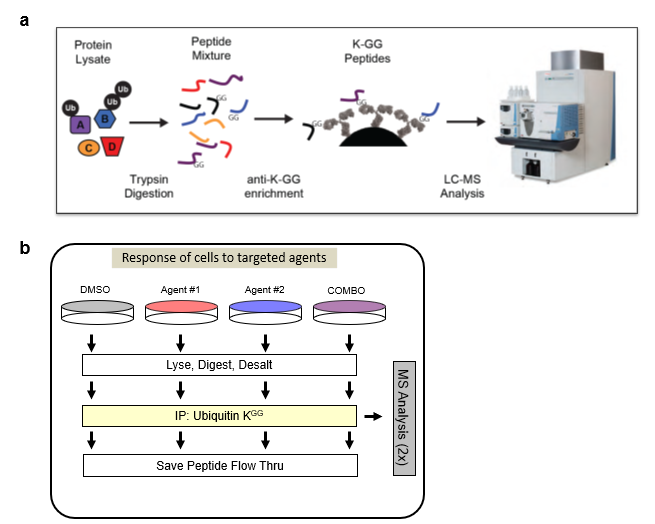
\includegraphics[scale=.8]{images/fig1.png}
\caption{\todo{Meena?: Write about how MS for PTMs is run?}}
\label{fig:workflow}
\end{figure}

\begin{figure}[ht]
\centering
\includegraphics[scale=.8]{images/fig3.png}
\caption{
Data structure of a typical PTM experiment and goals of PTM characterization. (a) Schematic data representation, in a simplified case of two conditions and two replicate runs. Each PTM site is modeled and characterized separately, where a PTM is quantified with multiple spectral features (boxes), distinguished by different charge states of a peptide. The feature intensities are viewed as repeated measurements of the underlying abundance of the PTM, where the abundance in Condition i is denoted by i. Features corresponding to unmodified peptides are considered together to perform adjustment with respect to protein abundance, where the protein abundance in Condition i is denoted by i*. Peptides can be fully cleaved (solid lines) and/or partially cleaved (dashed lines). Some spectral features can be missing. (b) PTM relative quantification by statistical inference, which makes use of the feature intensities to infer the underlying PTM abundance and protein abundance with an estimate of associated uncertainty. (c) Model-based testing for differential PTM abundance, which corrects for the underlying protein abundance with a cost of increased uncertainty about the estimate of difference between conditions.}
\label{fig:data-structure}
\end{figure}

\begin{figure}[ht]
\centering
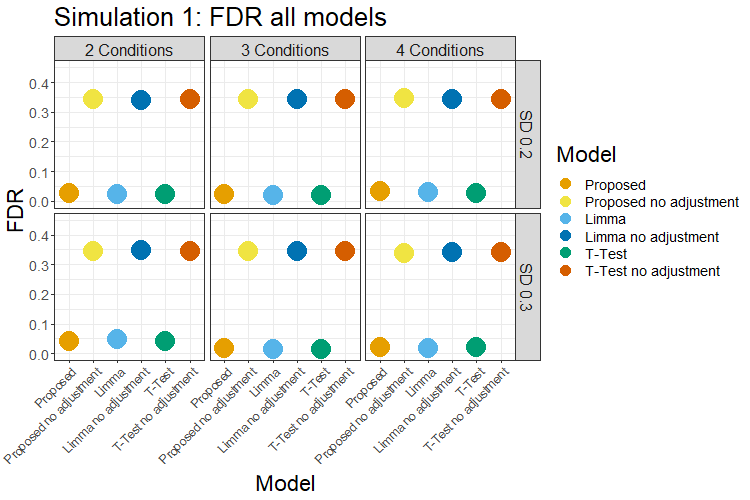
\includegraphics[width=1\textwidth]{images/sim1_FDR_all_models.png}
\caption{All the considered methods in simulation 1 correctly calibrated FDR when adjusting for changes in protein abundance. In comparison, the methods without accounting for the protein-level changes resulted in off-target, high false positive rates.
}\label{fig:fdr_all_models}
\end{figure}

\begin{figure}[ht]
\centering
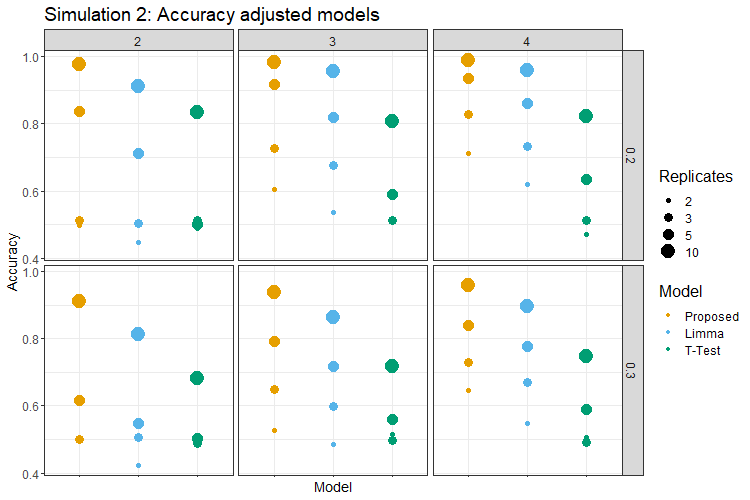
\includegraphics[width=1\textwidth]{images/sim3_Accuracy.png}
\caption{The advantage of using the proposed approach is apparent when looking at simulation 2, which includes limited observations and the presence of missing values. In overall accuracy, the proposed method performs stronger than Limma and t-test in nearly every model. Even at lower replicates the proposed method still outperformed Limma. The lowest performaning method was $t$-test. Limma shows comparable performance to the proposed method in a clean experiment, however when real world data problems are introduced it is clear the proposed method is more robust.}
\label{fig:sim_accuracy}
\end{figure}

\begin{figure}[ht]
\centering
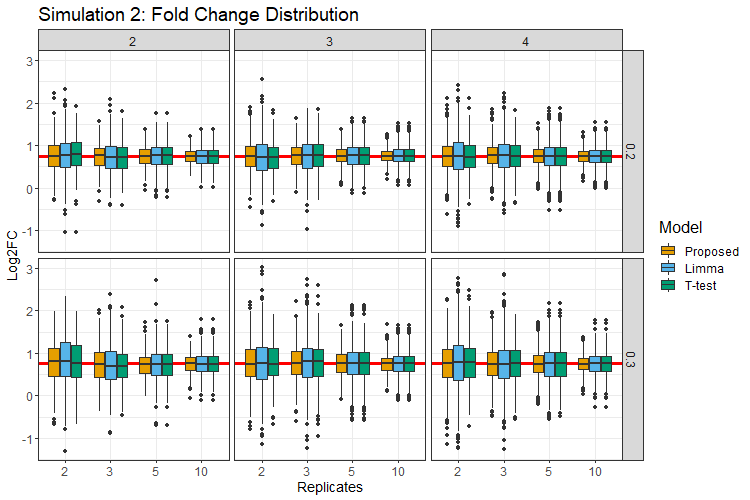
\includegraphics[width=1\textwidth]{images/sim3_FC_boxplot.png}
\caption{In the second simulation with missing values and low PTM features all methods correctly estimated the fold change with a median log change of .75. The proposed method in this simulation had a visibly tighter distribution around the median when compared to Limma and $t$-test. While the mean estimated fold changes were similar, the proposed method exhibited a stronger performance in correctly estimating the fold change for all peptides.}
\label{fig:sim_boxplot}
\end{figure}


\begin{figure}[ht]
\centering
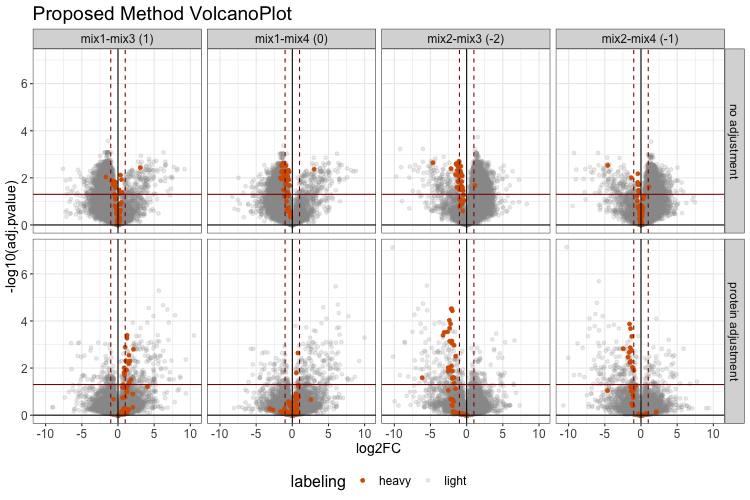
\includegraphics[width=1\textwidth]{images/spike_in_msstatsptm_volcano.png}
\caption{Using the proposed method to model the benchmark experiment the spike in peptides (colored red) do not follow the expected log fold change before adjustment. After adjusting for changes in overall protein abundance the spike in peptides are more in line with expectation. Additionally the background grey colored peptides showed many false positives before adjustment. After adjustment the false positives were decreased considerably.
}\label{fig:spikein_prop_volcano}
\end{figure}

\begin{figure}[ht]
\centering
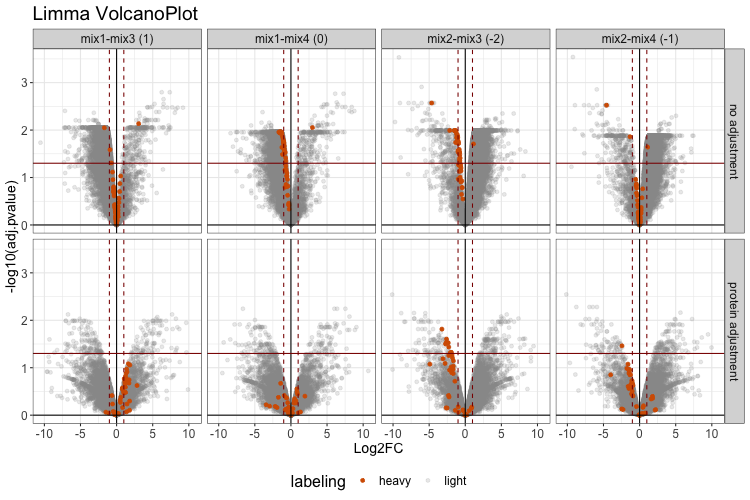
\includegraphics[width=1\textwidth]{images/spike_in_limma_volcano.png}
\caption{Limma method used to model the spike in experiment. Using Limma the spike in peptides follow the expected log fold change better after adjusting for changes in protein level. However, while the fold change is much more accurate, the majority of spike in peptides do not have a significant adjusted pvalue. In terms of false positives, the results are very similar to the proposed method, with many false positives before adjustment and much fewer after.
}\label{fig:spikein_limma_volcano}
\end{figure}

\begin{figure}[ht]
\centering
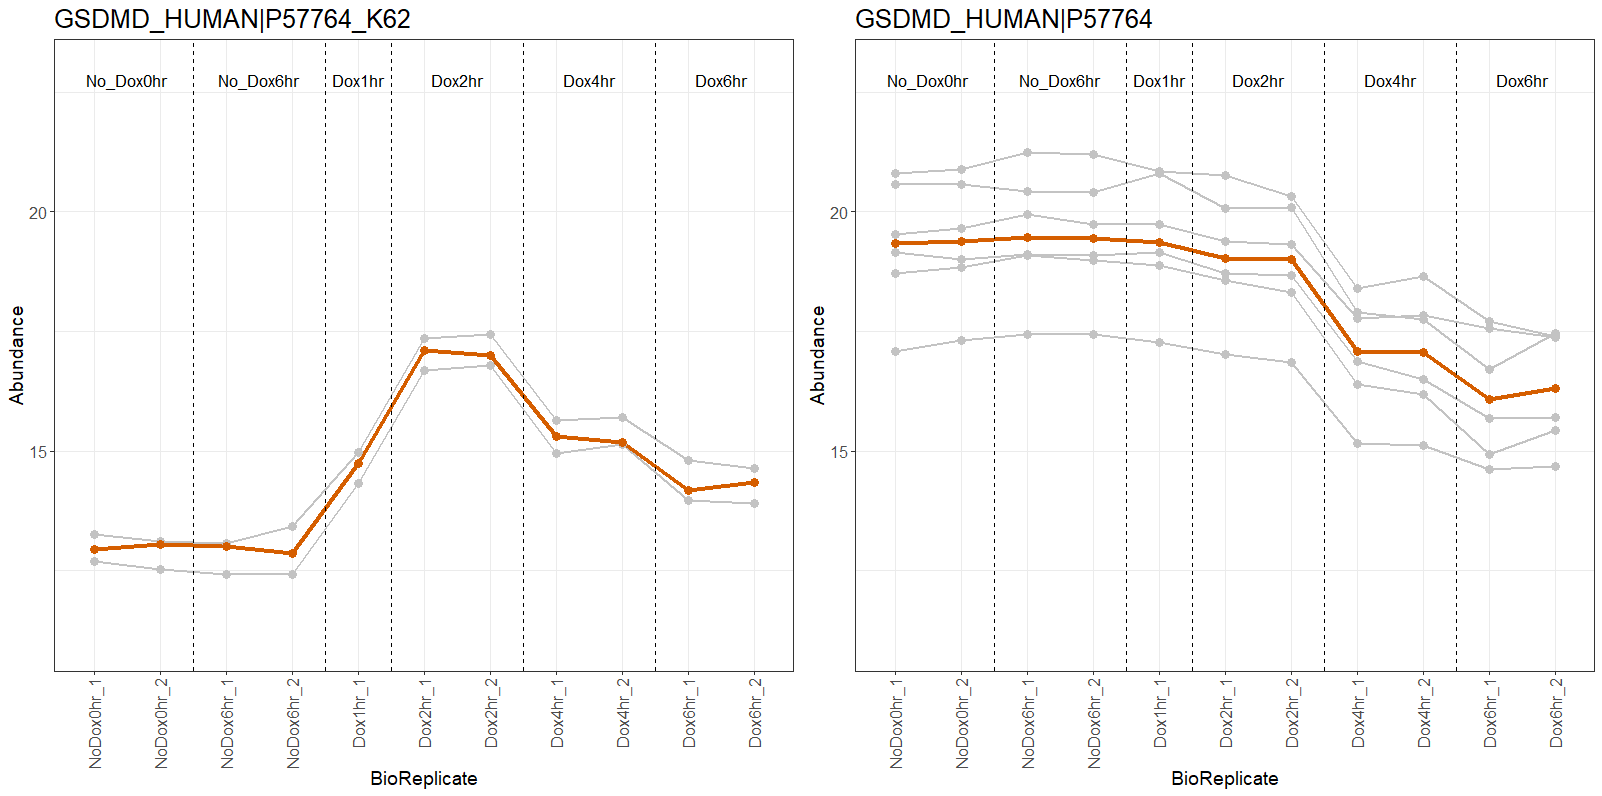
\includegraphics[width=1\textwidth]{images/IpaH_prof_plot.png}
\caption{The overlap of differencial modified peptides for the PTM model with and without global protein level adjustment. More PTMs became insignificant after adjustment then became significant. For the peptides that became insignificant in the adjusted model, their change in abundance was mainly due to changes in global protein abundance. In contrast, for peptides that became significant after adjustment, their true abundance change was masked by underlying changes in the unmodified protein.}
\label{fig:ipah_venn_diagramm}
\end{figure}

\begin{figure}[ht]
\centering
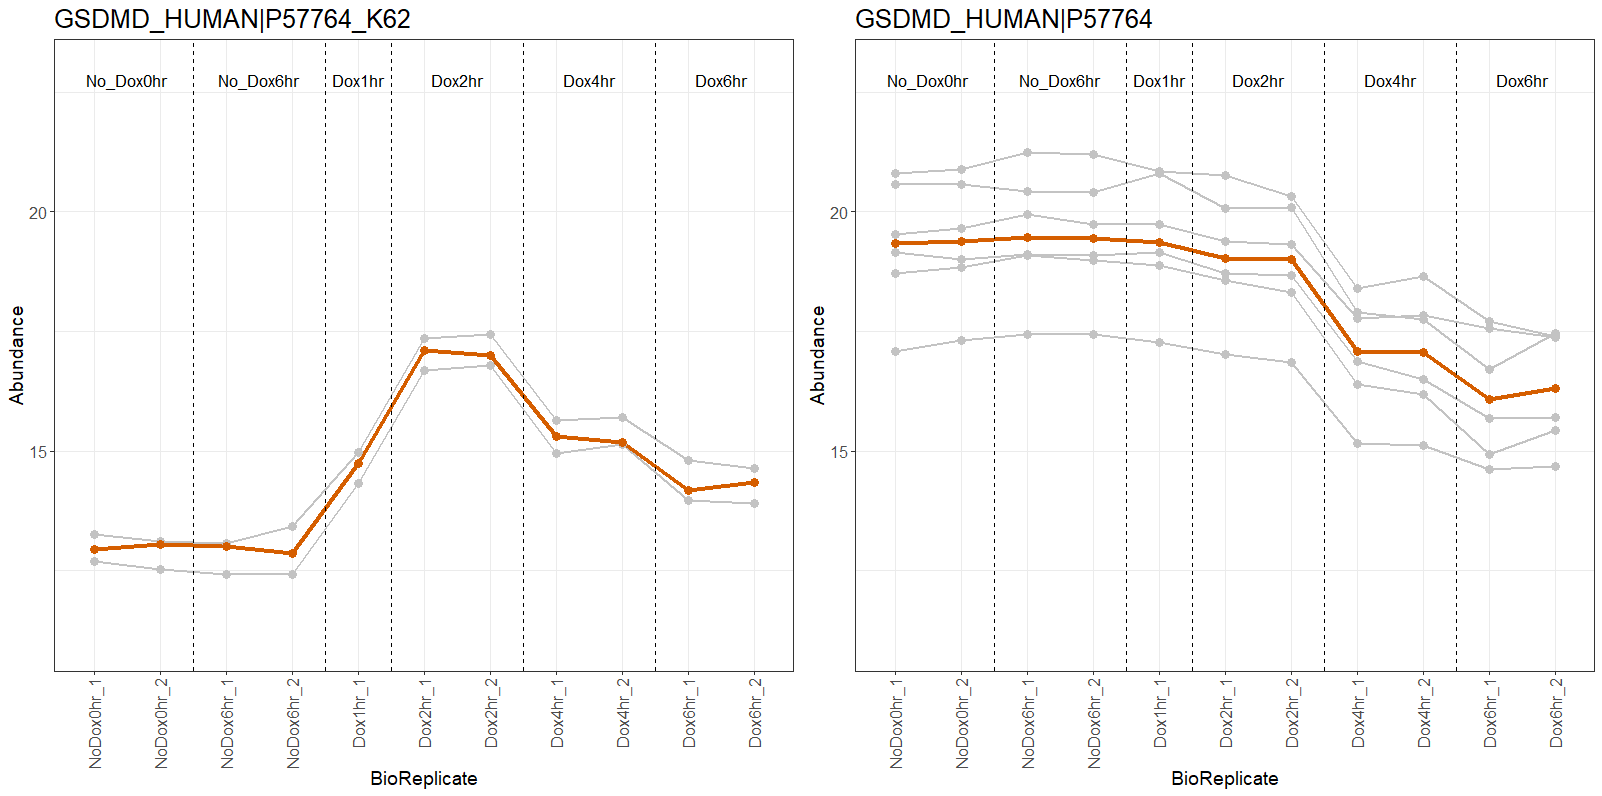
\includegraphics[width=1\textwidth]{images/IpaH_prof_plot.png}
\caption{Comparing the global profiling of protein $GSDMD\_HUMAN|P57764$ with the ubiquitination of the protein at site $K62$. The individual PSM features are shown in grey, while the feature summarization is shown in red. When looking at the summary of the modification and global protein it is clear the conditions follow different trends. Specifically, there appears to be no change in abundance between Dox1hr and Dox4hr in the modified plot, however there is a large negative change when looking at the unmodified plot. This indicates the modification is confounded with changes in the unmodified protein.}
\label{fig:ipah_profile}
\end{figure}

\begin{figure}[h!]
\centering
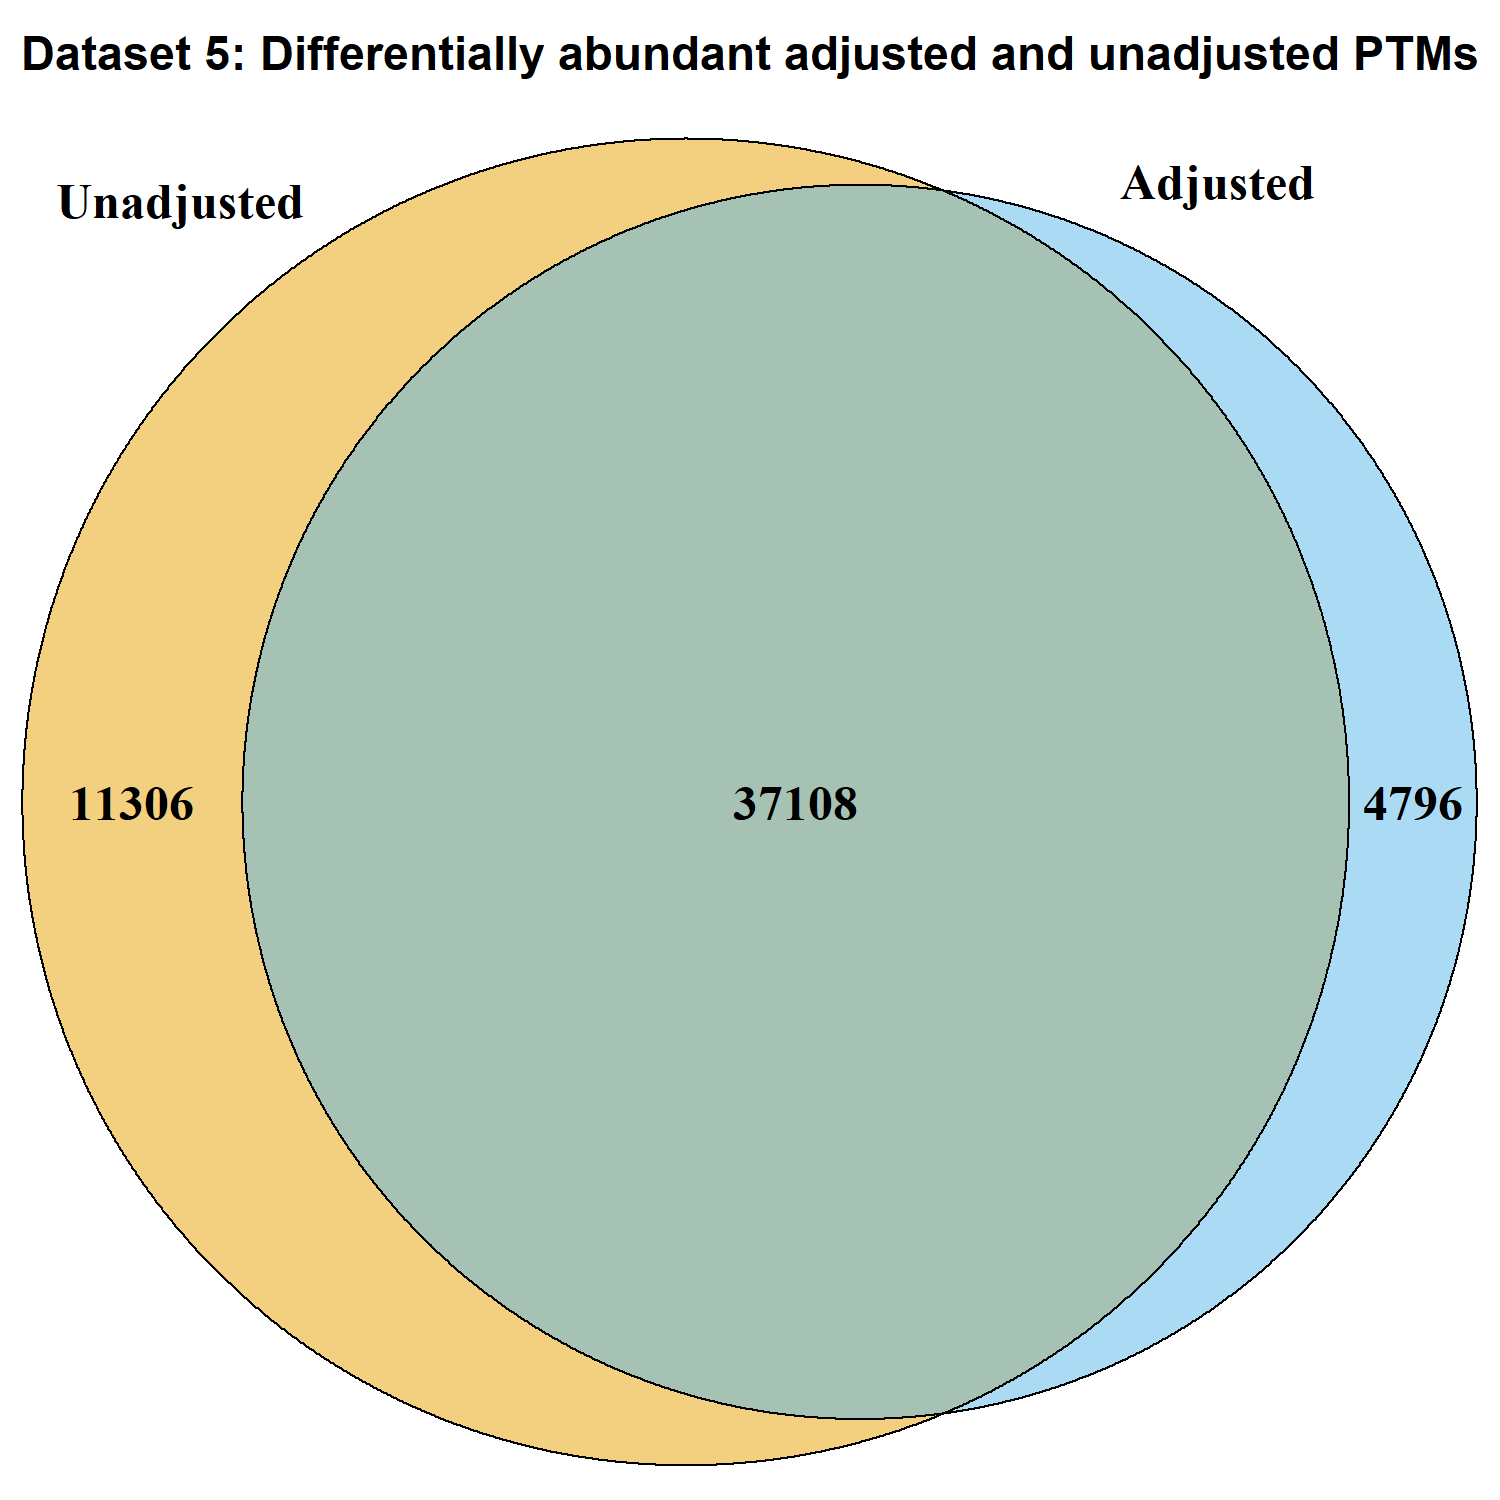
\includegraphics[height=.65\textwidth]{images/shig_venn_diagramm.png}
\caption{The overlap of differencial modified peptides between the PTM model with and without global protein level adjustment. Again more PTMs became insignificant after adjustment then became significant.}
\label{fig:shig_venn_d}
\end{figure}

\begin{figure}[h!]
\centering
\begin{subfigure}{\textwidth}
 \centering
	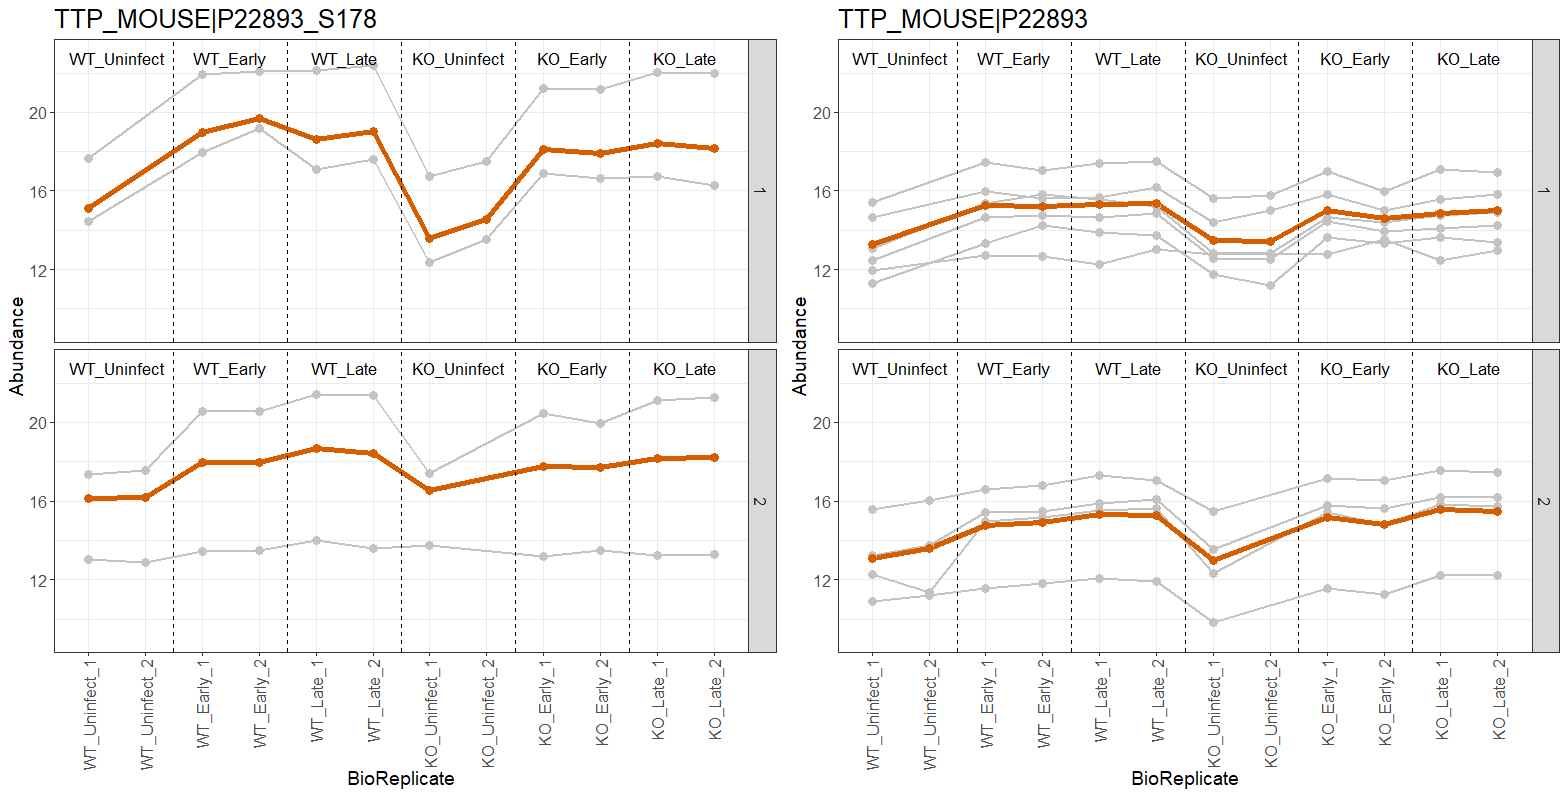
\includegraphics[width=.95\textwidth]{images/No_Difference_Shigella_Profile_Plot}
	\caption{Comparing the global profiling of protein $TTP\_MOUSE|P22893$ with the modification of the protein at site $S178$. The individual PSM features are shown in grey, while the feature summarization is shown in red. When looking at the summary of the modification and global protein it is clear the difference between conditions follow the same trend. Specifically, there is a positive adjustment in abundance when comparing WT\_Uninfect to WT\_Late in both the modification and global profiling run. This indicates the movement is driven by changes in global protein.}
 \end{subfigure}\vspace{5mm}
 \begin{subfigure}{\textwidth}
 \centering
	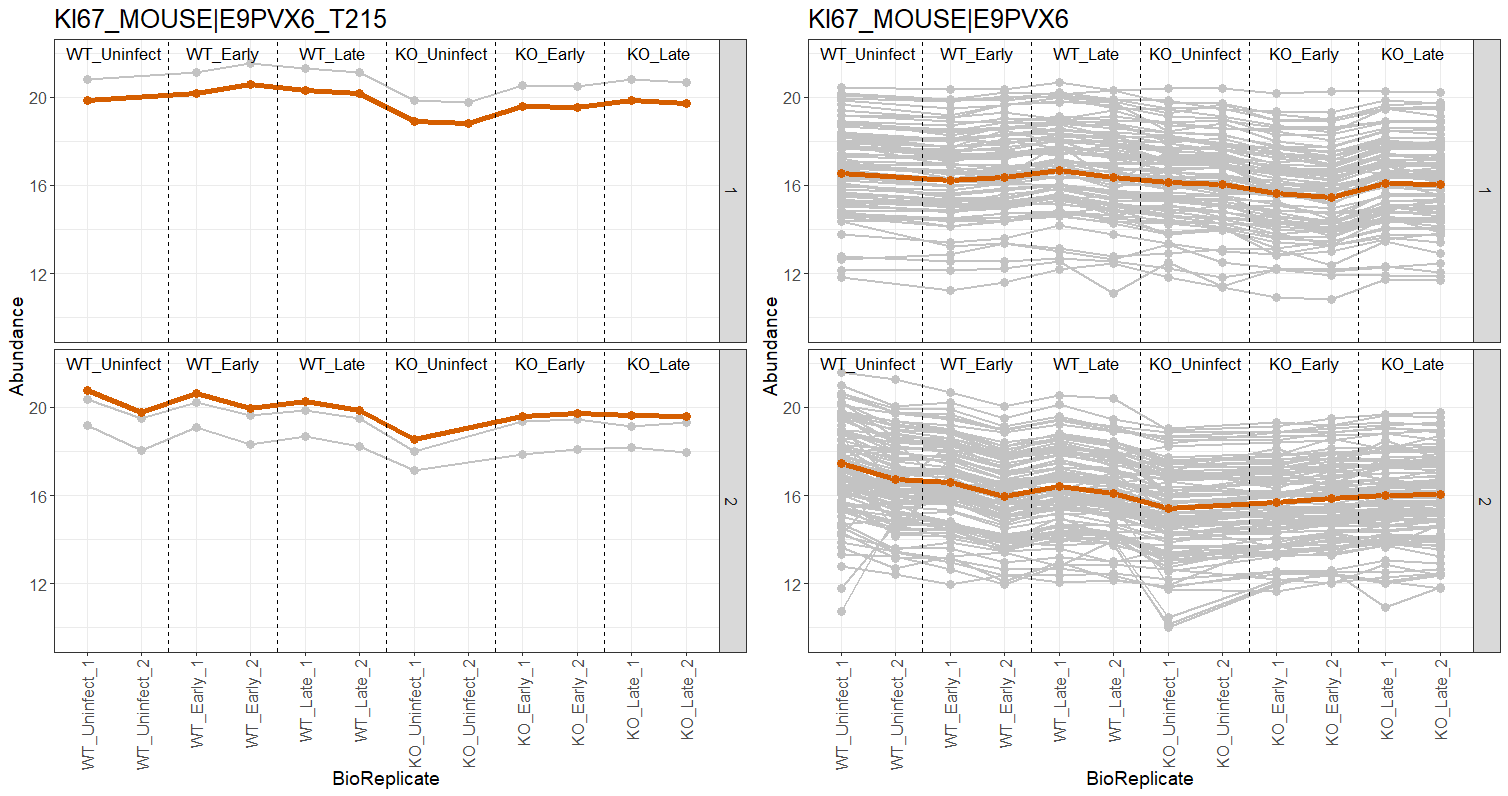
\includegraphics[width=.95\textwidth]{images/Difference_Shigella_Profile_Plot}
	\caption{Comparing the global profiling of protein $KI67\_MOUSE|E9PVX6$ with the modification of the protein at site $T215$. In this case the modification and global protein trend in different directions. Specifically, comparing WT\_Uninfect and WT\_Early there is a slightly positive change in abundance, however in the global profiling there was a negative change. In this case the profile plot indicates the effect of the modification is masked by the change in global protein abundance. Additionally this profile plot shows the large difference in available features between modifications and global protein.}
 \end{subfigure}
\caption{Profile plots for PTMs P22893\_S178 and E9PVX6\_T215 in the Shigella flexneri experiment.}
\label{fig:shigella_profile}
\end{figure}

\begin{figure}[h!]
\centering
 \begin{subfigure}{\textwidth}
 \centering
	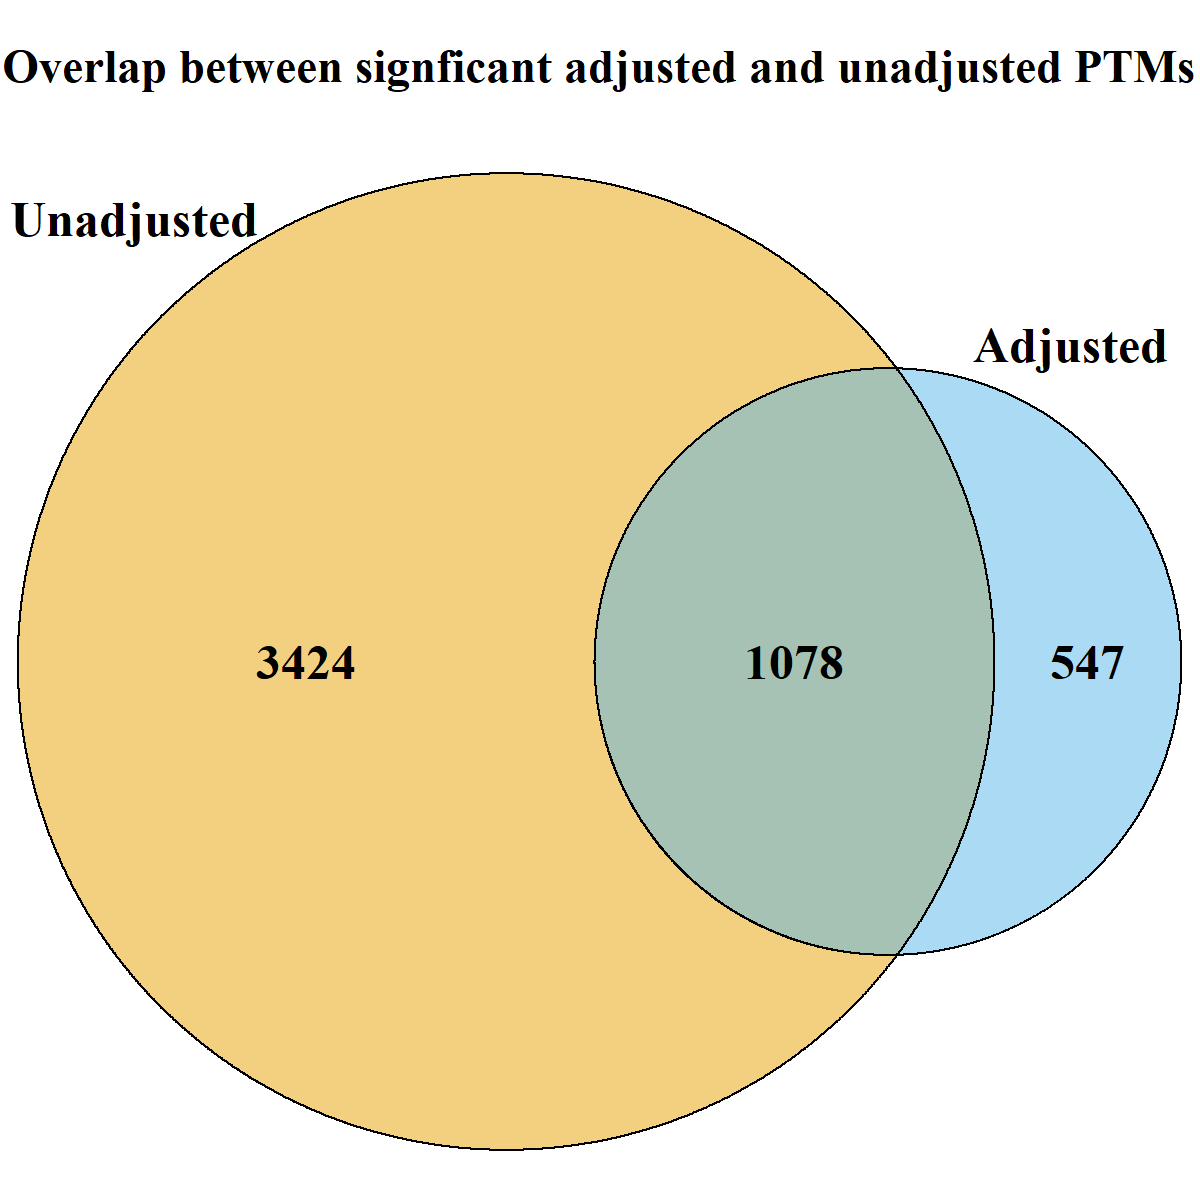
\includegraphics[height=.5\textwidth]{images/usp30_venn_diagramm}
	\caption{The overlap of differencial modified peptides for the PTM model with and without global protein level adjustment. Here many more PTMs became insignificant then became significant after adjustment. This is due to not having a global profiling run, resulting in a large lack of overlap between the modified peptides and unmodified proteins.}
 \end{subfigure}\vspace{-5mm}
 \begin{subfigure}{\textwidth}
 \centering
	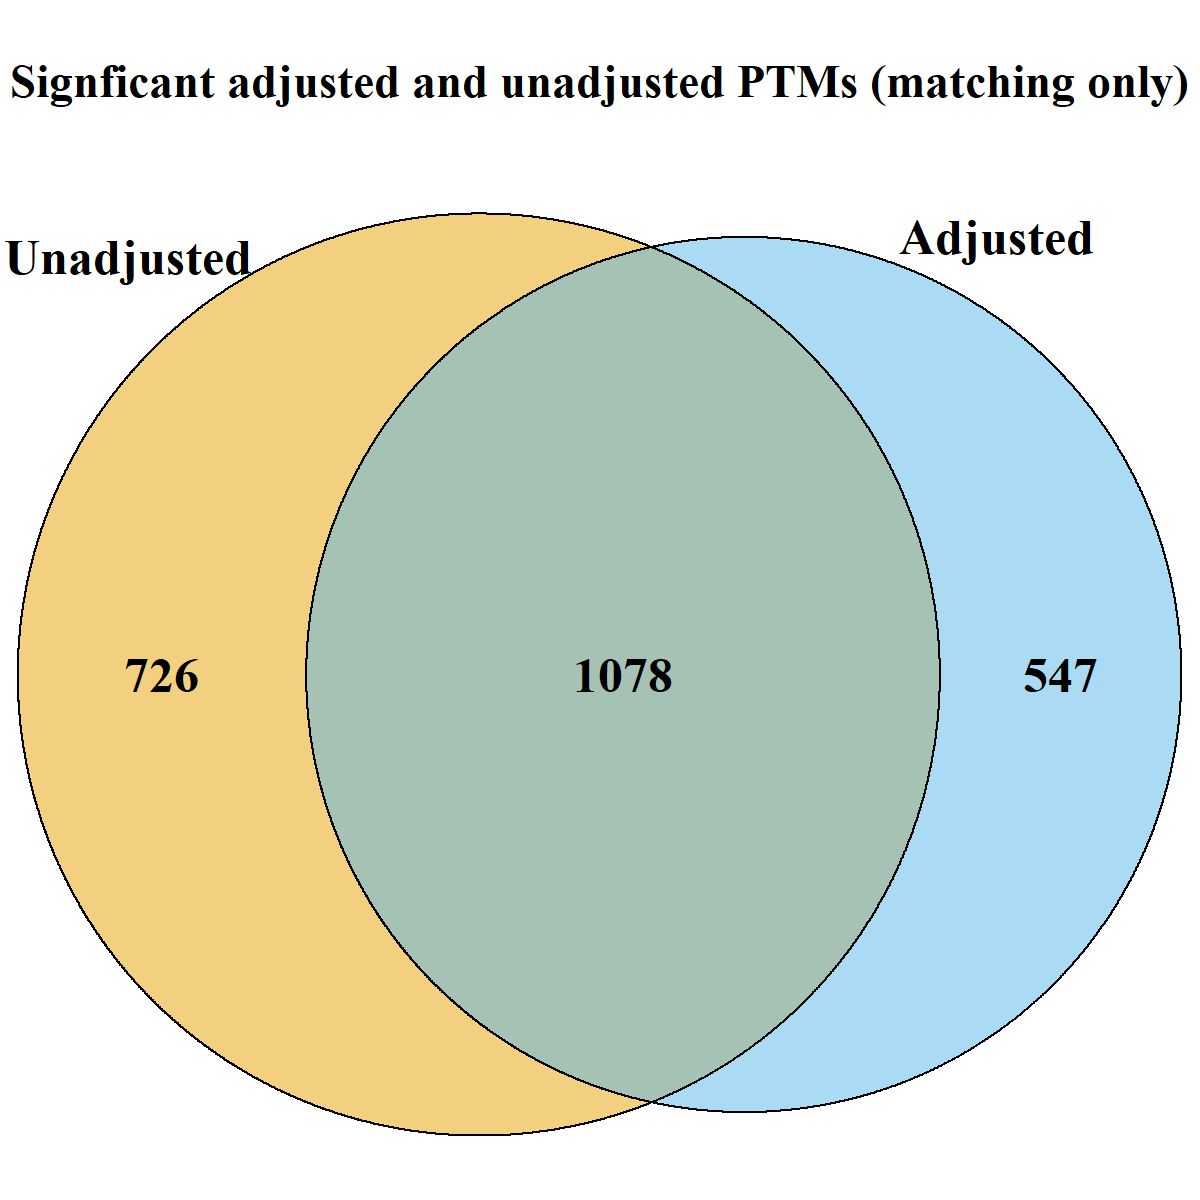
\includegraphics[height=.5\textwidth]{images/usp30_venn_diagramm_matching_only}
	\caption{Here we make the same comparison but only for modified peptides with a matching unmodified protein, so adjustment can be performed. In this case we see significantly less peptides become insignificant after adjustment. This highlights the need for a global profiling run if protein adjustment is going to performed.}
 \end{subfigure}
 \caption{Overlap of significant PTMs before and after protein adjustment.}
\label{fig:usp30_ven_d}
\end{figure}

\begin{figure}[ht]
\centering
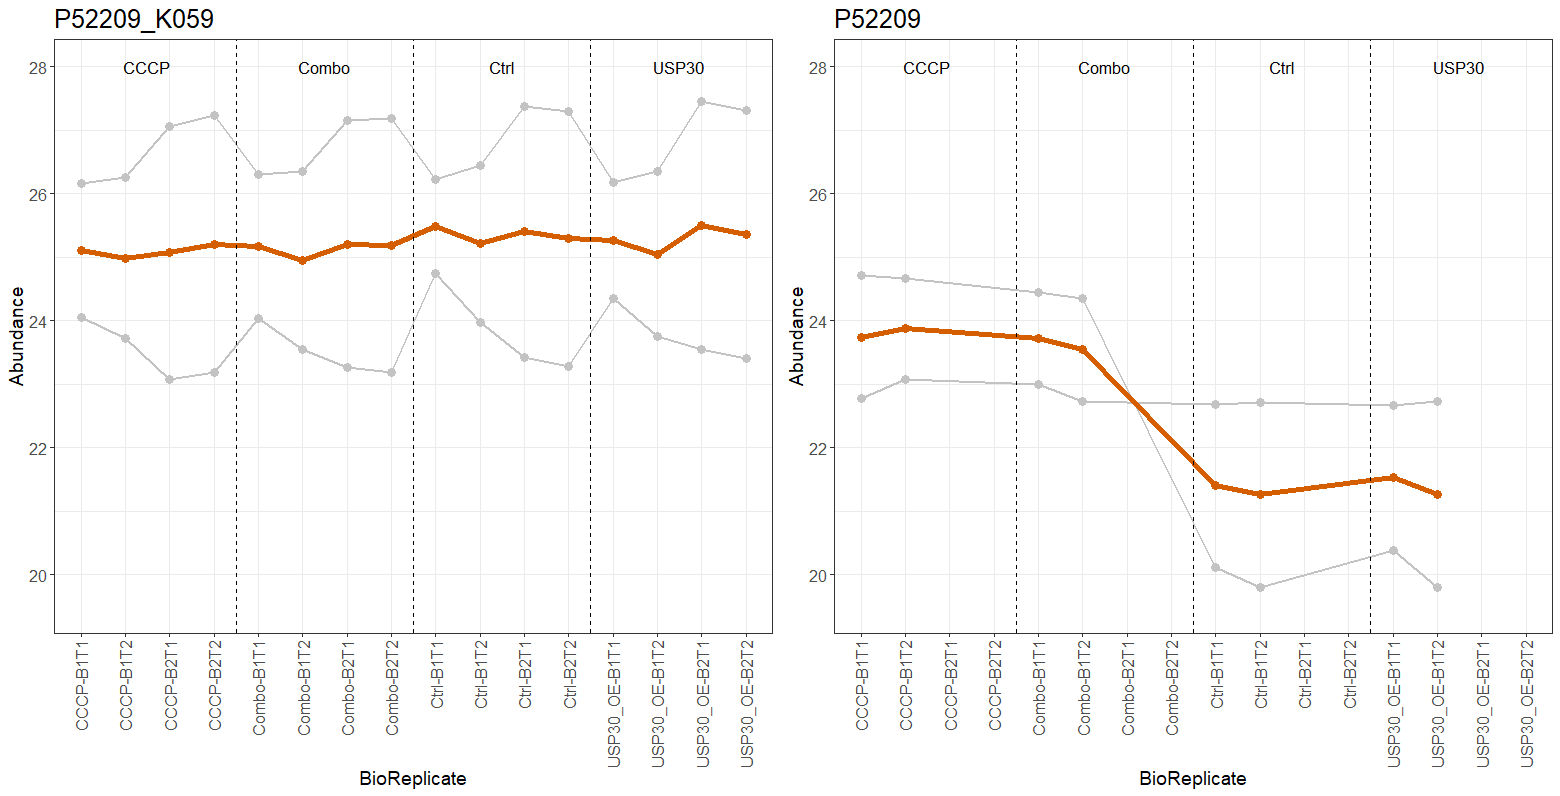
\includegraphics[width=1\textwidth]{images/USP30_profile_plot.png}
\caption{Comparing the global profiling of protein $P52209$ with the modification of the protein at site $K059$. The modification appears generally unchanged between conditions, whereas the global profiling run shows the CCCP and Combo conditions at a higher relative abundance compared to the Control and USP30\_OE. This indicates that the modification actually had a major effect when comparing CCCP and Combo to Control and USP30\_OE, which would have been missed without adjusting for global protein changes.}
\label{fig:usp30_profile}
\end{figure}

%{\bf Figure 4} False positive rate and statistical power in PTM significance analysis by the proposed approach, t-test with protein-level adjustment, and t-test without protein-level adjustment. (a) When there was no change in protein abundance, all considered methods well calibrated the Type I error rate. (b) When the PTM changes were entirely due to changes in protein abundance across conditions, analysis accounting for the protein-level changes resulted in off-target, high false positive rates. (c) Statistical powers by the proposed approach and t-test with protein-level adjustment, where the data consisted of 2 conditions and the SD corresponding unmodified feature intensities was 0.2. (d) Statistical powers by the proposed approach and t-test with protein-level adjustment, where the data consisted of 2 conditions, the SD corresponding unmodified feature intensities was 0.2, and the PTM was missing in Run 1 of Condition 1. (e) Same as in (d), but the data consisted of 4 conditions.

%{\bf Figure 5} Results corresponding to estimation error and false positive rate and statistical power of the PTM significance analysis, where the data were acquired in two batches. The following parameters were considered to represent the batch effects: no batch-condition interaction, mean intensity level in Batch 2 was higher than Batch 1 by 2 on log scale, and the SDs in Batch 1 and Batch 2 were 0.2 and 0.3, respectively.(a)Estimation based on the most statistically significant batch with t-test was more variable than other methods and frequently biased. (b)The proposed approach better calibrated Type I error rate. (c)The proposed approach improved statistical power in all the considered cases with different number of conditions and replicates. This was achieved by properly characterizing batch effects and leveraging all available information. Ignoring batch effects by t-test (no batch) lost power dramatically. The negative impact was only partially reduced by increasing the sample size to 5.

%{\bf Figure 6} Design of future PTM experiments in terms of sample size calculations and power analysis. (a) Protein-level adjustment relies on the inference of protein abundance, which introduces additional uncertainty in the estimate of PTM difference. Therefore, the required sample size to detect a systematic change is higher than as expected for standard differential analysis without adjustment. Sample size calculations without accounting for the uncertainty would lead to over-optimistic, under-powered studies. (b) In complex designs, simultaneously analyzing all the conditions effectively increases the degrees of freedom and requires fewer replicates. (c)Increasing the sample size and analyzing multiple conditions together both result in improved statistical power.


\end{document}
